\documentclass{beamer}

\usepackage{pgf,pdfpages}

\mode<presentation>
{
    \usetheme{bunsen}
    \setbeamercovered{transparent}
    \setbeamertemplate{items}[circle]
}

% suppress navigation bar
\beamertemplatenavigationsymbolsempty

\usefonttheme[onlymath]{serif}
\setbeamerfont{frametitle}{size=\LARGE,series=\bfseries}

\defbeamertemplate{enumerate item}{mycircle}
{
    \begin{pgfpicture}{0ex}{0ex}{1.5ex}{0ex}
        \pgfbox[center,base]{\insertenumlabel.}
    \end{pgfpicture}
}
[action]
{\setbeamerfont{item projected}{size=\scriptsize}}
\setbeamertemplate{enumerate item}[mycircle]

%% SPACING BETWEEN ITEMS FOR BEAMER
%% following lets me add length between items
%% http://tex.stackexchange.com/questions/16793/global-setting-of-spacing-between-items-in-itemize-environment-for-beamer
% \let\oldframe\frame
% \renewcommand{\frame}{
% \oldframe
% \let\olditemize\itemize
% %%\renewcommand\itemize{\olditemize\addtolength{\itemsep}{0.5\baselineskip}}
% \renewcommand\itemize{\olditemize\addtolength{\parskip}{0.5\baselineskip}} %% this affects nested list (itemize) as well
% }
\newlength{\wideitemsep}
\setlength{\wideitemsep}{\itemsep}
\addtolength{\wideitemsep}{0.5\baselineskip}
\let\olditem\item
\renewcommand{\item}{\setlength{\itemsep}{\wideitemsep}\olditem}
%%\usepackage{enumitem} %% traditional way to modify listing (itemize and enumerate) properties...but beamer has its own definition
%% NESTED LISTS
%% http://tex.stackexchange.com/questions/20654/length-between-nested-lists
\setbeamertemplate{itemize/enumerate subbody begin}{\vspace{0.5\baselineskip}}
\setbeamertemplate{itemize/enumerate subbody end}{\vspace{0.5\baselineskip}}
%% MORE OPTIONS http://tex.stackexchange.com/questions/11168/change-bullet-style-formatting-in-beamer

\title{Sega Game Gear on a Chip}
\author{Max Thrun | Samir Silbak}
\institute{University of Cincinnati}
\date{Fall 2012}

\begin{document}

\maketitle

%
% background for the rest of the slides
%
\setbeamertemplate{background}
{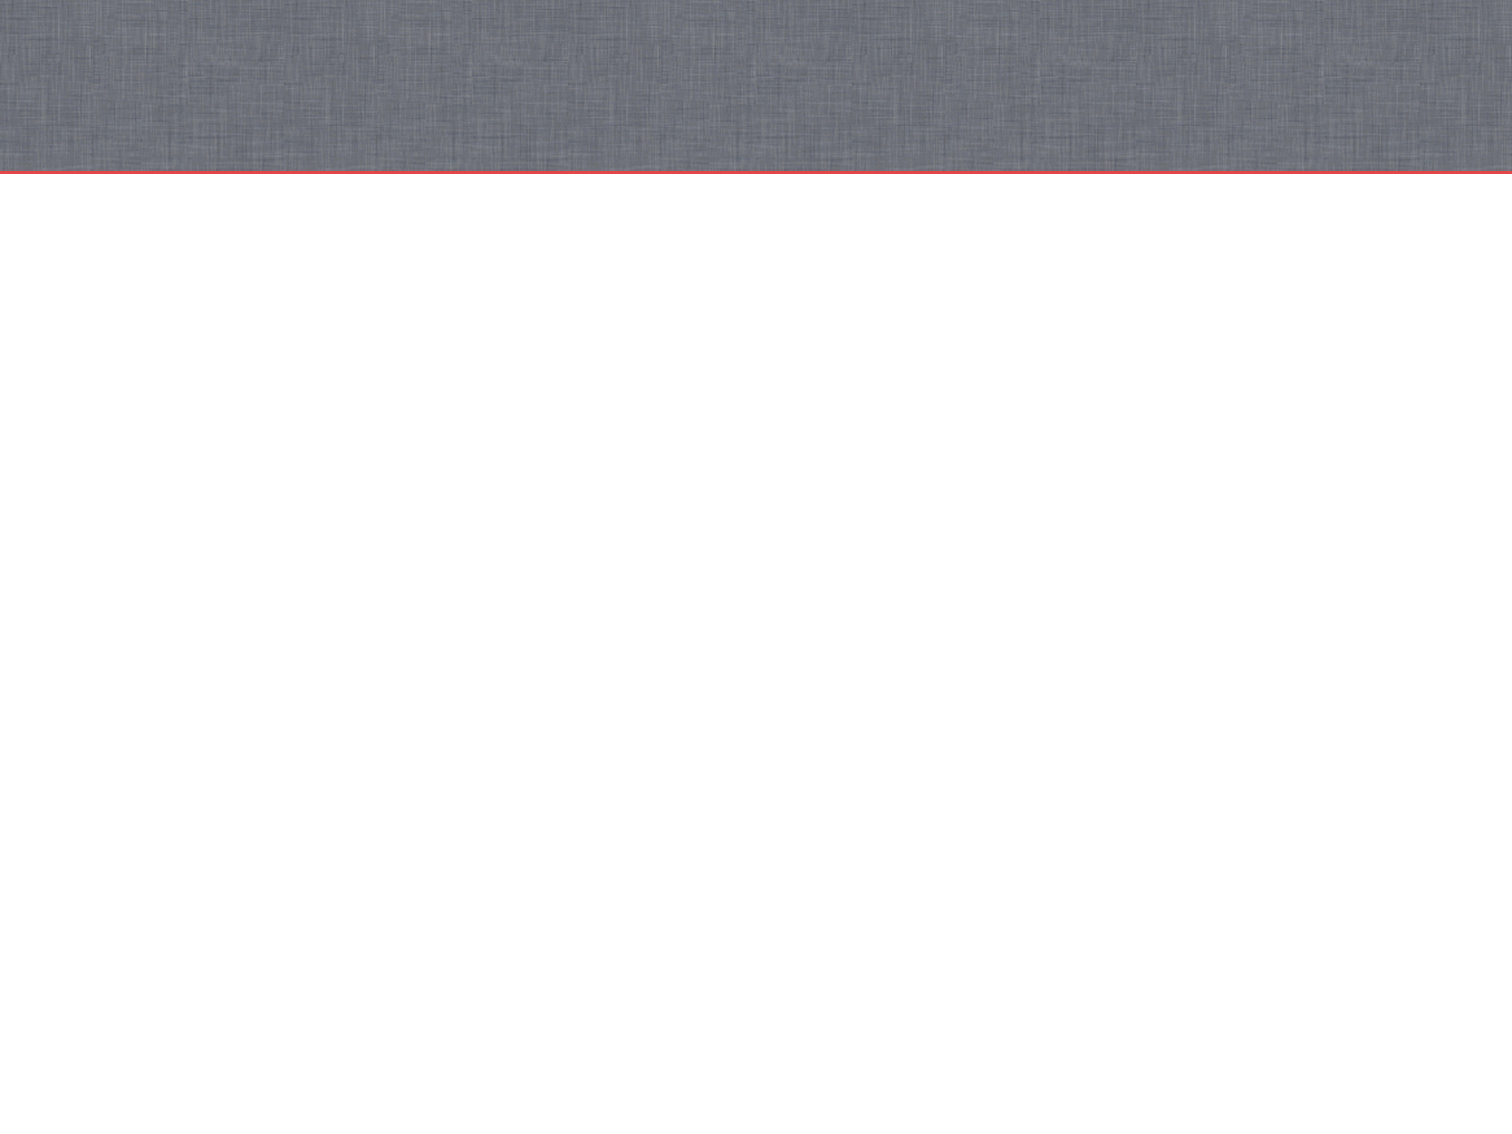
\includegraphics[width=\paperwidth,height=\paperheight]{slide_bg}}
\setbeamertemplate{footline}[bunsentheme]

\section{Agenda}
\begin{frame}
\frametitle{Agenda}
    \begin{itemize}
        \item Introduction / Problem Description
        \item The Sega Game Gear
        \item Prototyping Platform
        \item Design Strategy \& Process
        \item Component Descriptions
        \item Testing Strategy / Assessment Metrics
        \item Issues of Concern
    \end{itemize}
\end{frame}

\section{Introduction}
\begin{frame}
\frametitle{Underlying Goal}
    \begin{center}
        \Large
        Reimplement all the digital components of \\a legacy computer system in a FPGA
    \end{center}
\end{frame}

\begin{frame}
    \frametitle{Purpose}

    \begin{columns}[c]
        \column{0.6\textwidth}
            Why?
            \begin{itemize}
                \item<2-> \textbf{Maintainability} - You can no longer buy parts to service legacy computer systems
                \item<3-> \textbf{Upgradability} - Reimplementation gives an opportunity to add additional features
                \item<4-> \textbf{Portability} - Do not need all the original big clunky hardware. Reimplementation can
                    be embedded in new designs
            \end{itemize}

        \column{0.4\textwidth}
            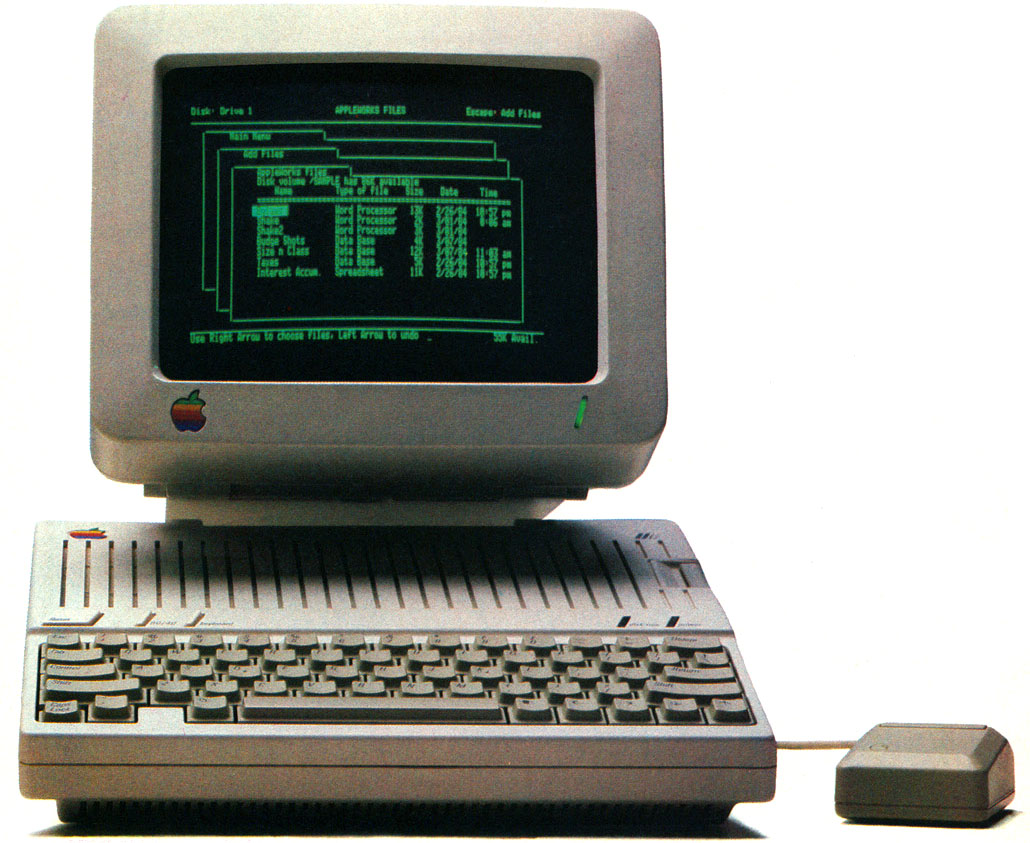
\includegraphics[width=\textwidth]{apple_2.jpg}
    \end{columns}
\end{frame}

\section{Sega Game Gear}
\begin{frame}
    \frametitle{Sega Game Gear}
    \begin{center}
        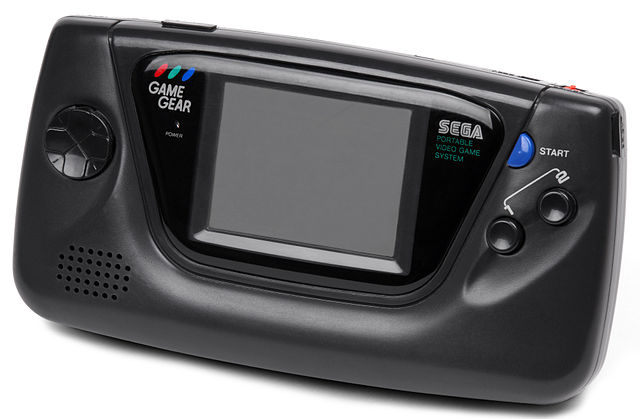
\includegraphics[width=0.6\textwidth]{gg.jpg}
    \end{center}
\end{frame}

\begin{frame}
    \frametitle{Sega Game Gear}

    \begin{columns}[c]
        \column{0.5\textwidth}
            \begin{itemize}
                \item Released April 1990
                \item Mobile version of the Sega Master System (functionally identical)
                \item Standard system architecture for the time (Z80 CPU, tri-state buses, etc...)
            \end{itemize}

        \column{0.5\textwidth}
            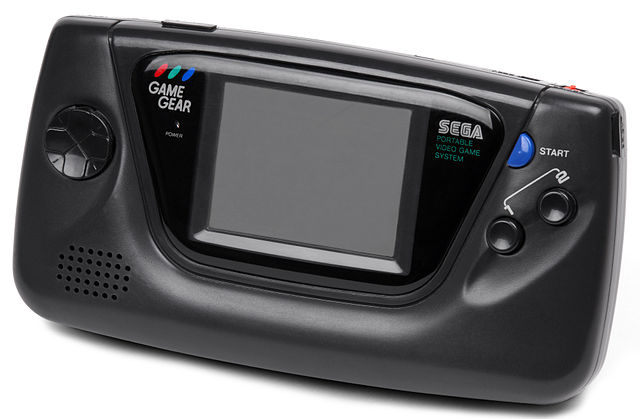
\includegraphics[width=\textwidth]{gg.jpg}
    \end{columns}
\end{frame}

\begin{frame}
    \frametitle{Sega Master System PCB}
    \begin{center}
        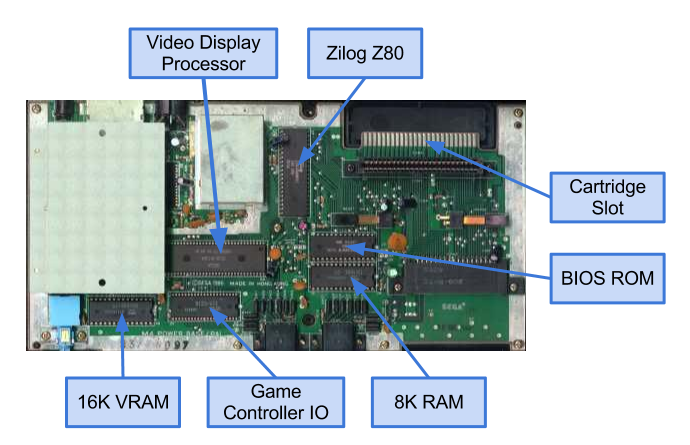
\includegraphics[width=\textwidth]{sms_pcb.png}
    \end{center}
\end{frame}

\begin{frame}
    \frametitle{Black Box Diagram}
    \begin{center}
        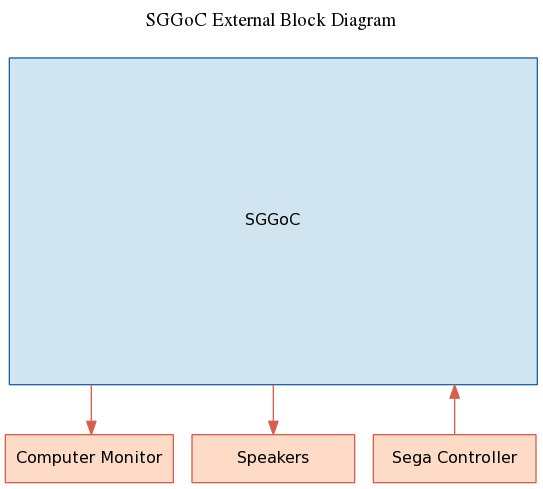
\includegraphics[width=\textwidth]{../block_diagrams/block_diagram_external.png}
    \end{center}
\end{frame}

\begin{frame}
    \frametitle{Transparent Box Diagram}
    \begin{center}
        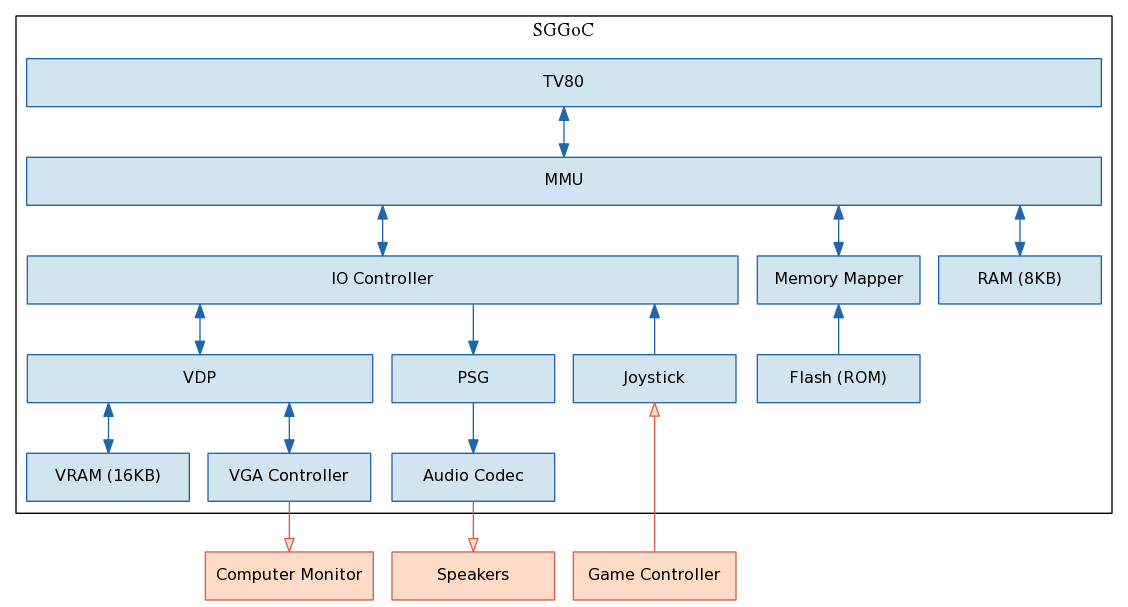
\includegraphics[width=\textwidth]{../block_diagrams/block_diagram_internal.png}
    \end{center}
\end{frame}

\section{Prototyping Platform}
\begin{frame}
    \frametitle{FPGA Development Board}
    \begin{center}
        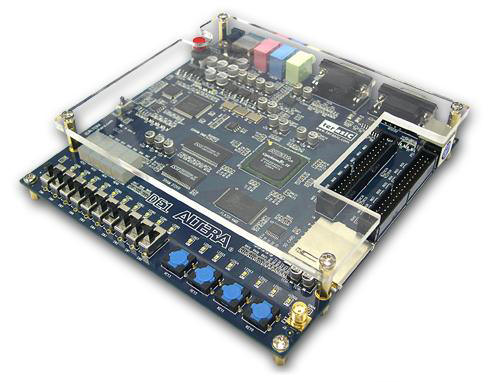
\includegraphics[height=0.7\textheight]{de1_angle.jpg}
    \end{center}
\end{frame}

\begin{frame}
    \frametitle{Altera DE1}

    \begin{columns}[c]
        \column{0.5\textwidth}
            \begin{itemize}
                \item Cyclone II EP2C20F484C7
                \item VGA, Audio, SD Card, 4 MB Flash
                \item Supports a familiar command line development environment
                \item Extremely good documentation
            \end{itemize}

        \column{0.5\textwidth}
            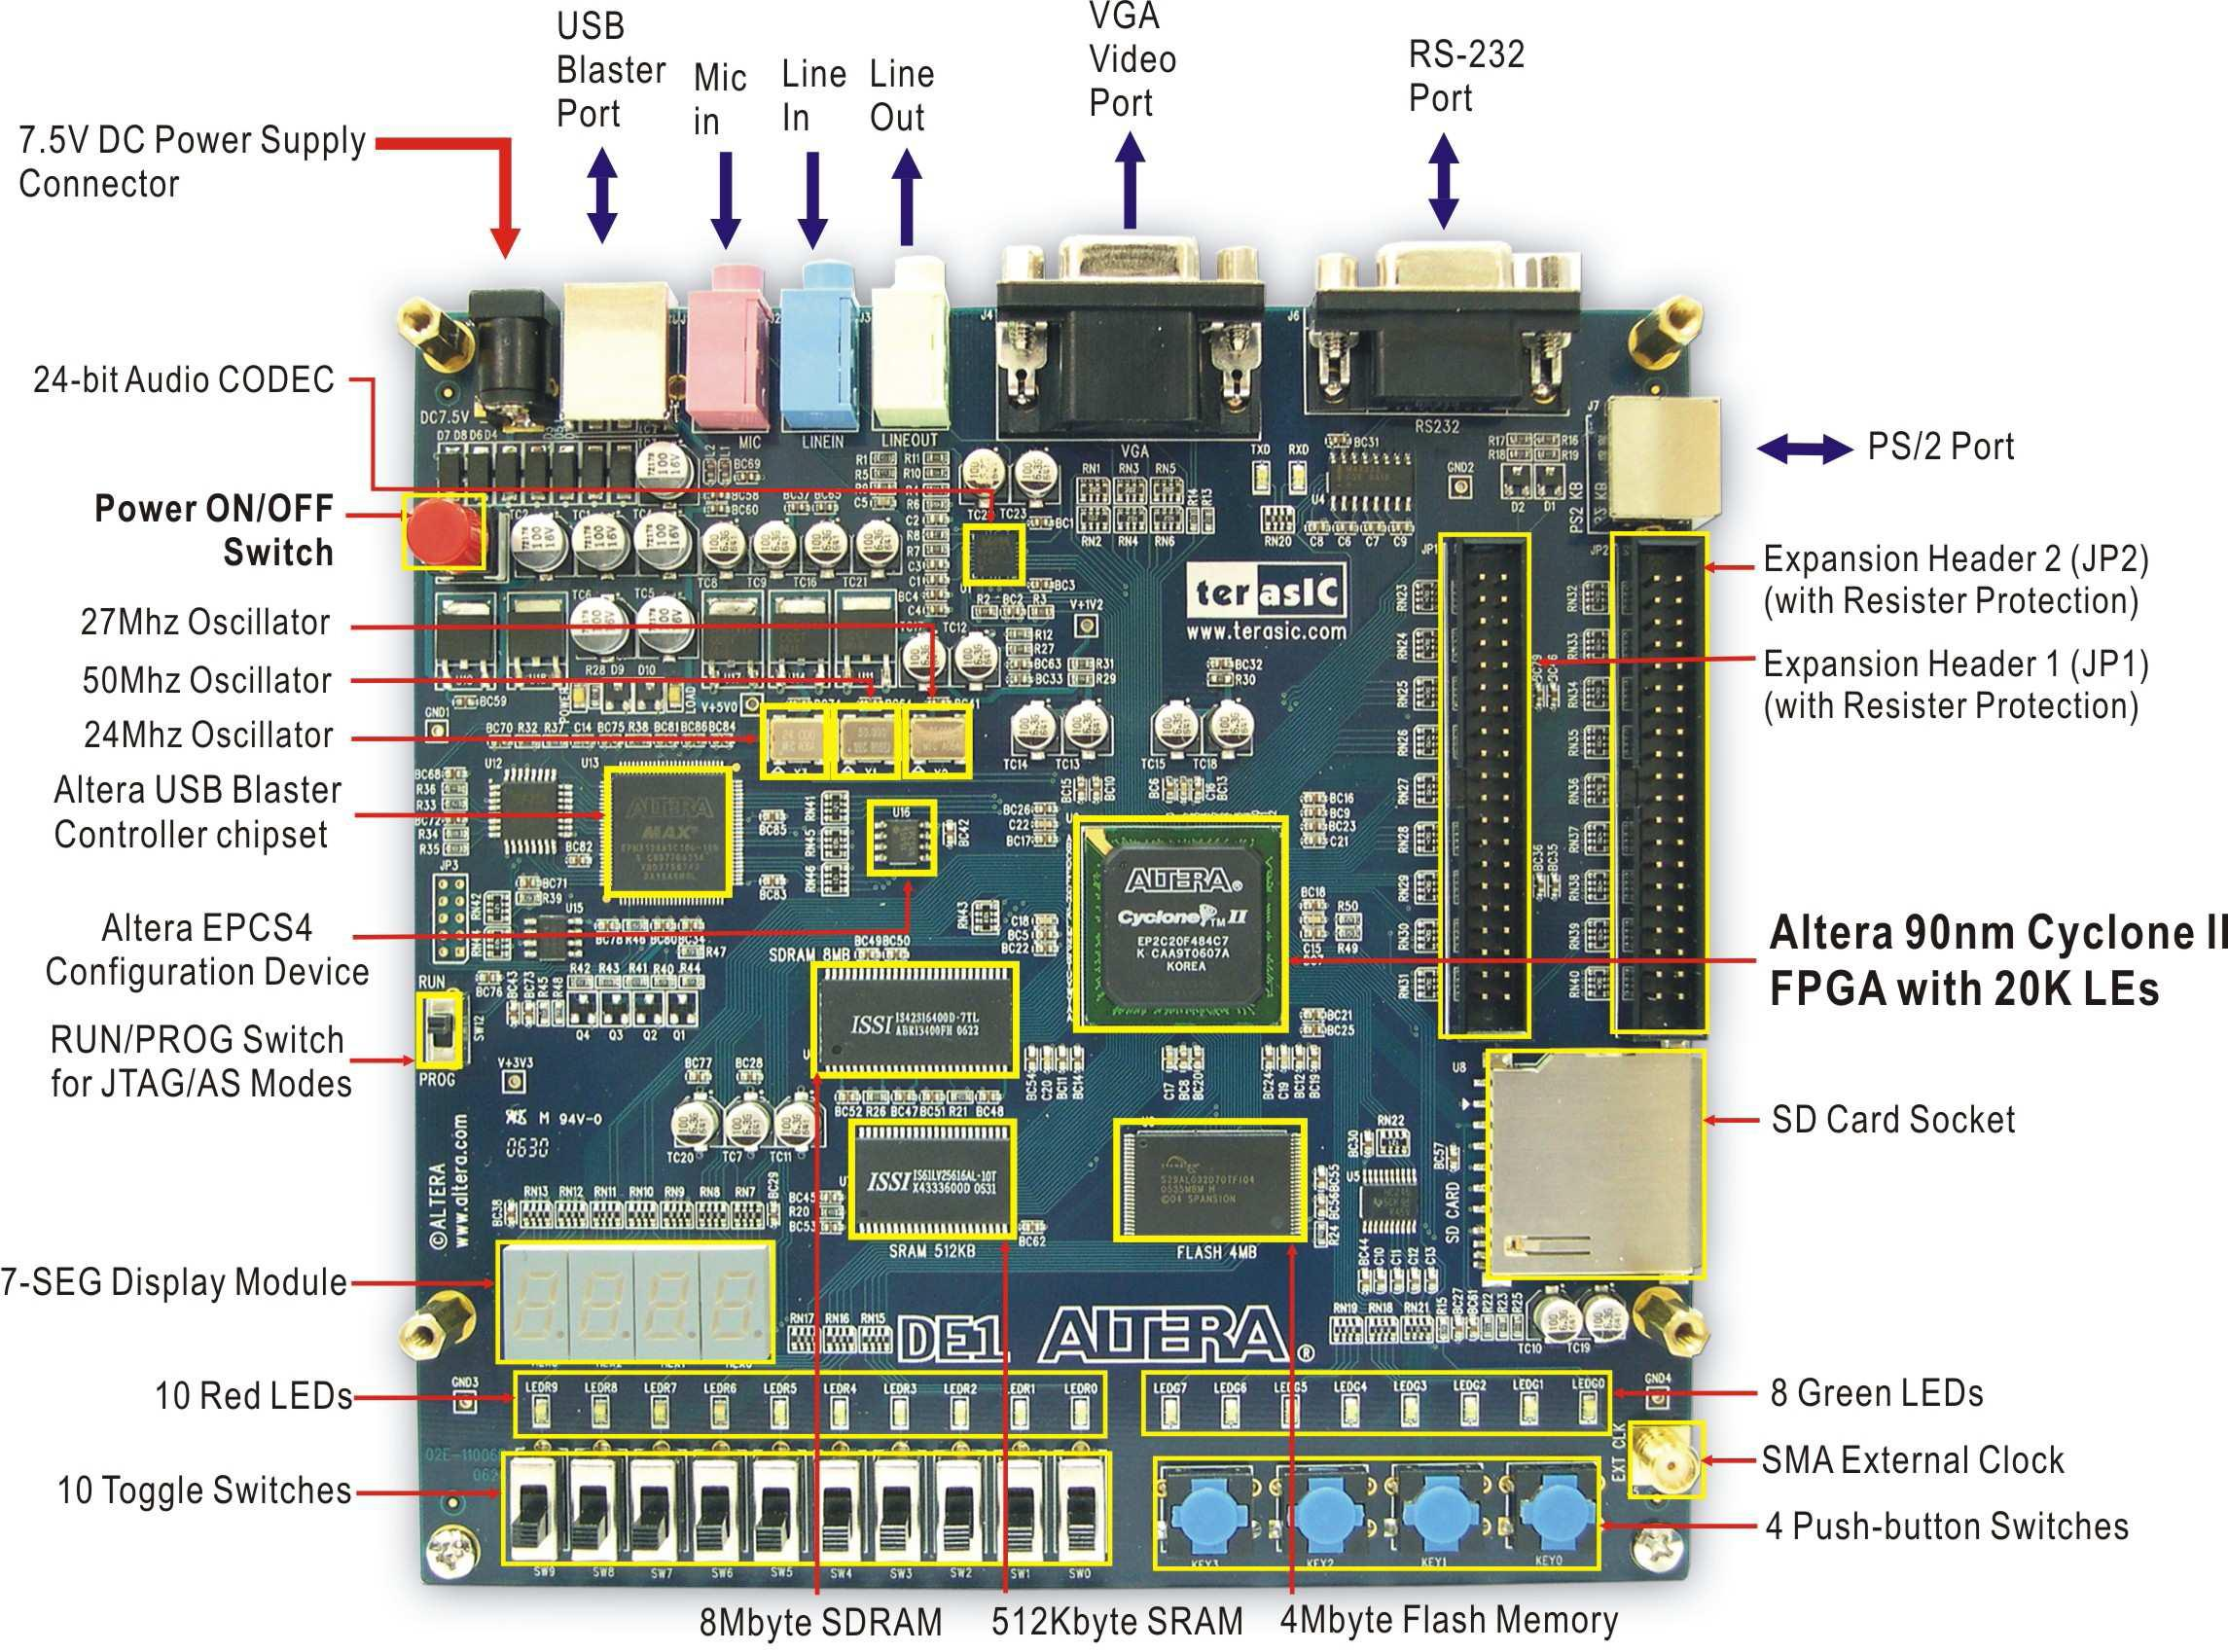
\includegraphics[width=\textwidth]{de1.jpg}
    \end{columns}
\end{frame}

\section{Design Strategy}
\begin{frame}
    \frametitle{Design Strategy}
    \begin{enumerate}
        \item<1-> Break down system components according to the original system architecture
        \item<2-> Implement each component to match the original functionality described by official and
            non official documents
        \item<3-> Test each components functionality against the actual hardware (in our case an emulator)
        \item<4-> Tie components together in a way that is better suited toward FPGA technology (\emph{E.g.} avoid tri-state buses)
    \end{enumerate}
\end{frame}

\section{Component Descriptions}
\begin{frame}
    \frametitle{Game Cartridge}
    \begin{center}
        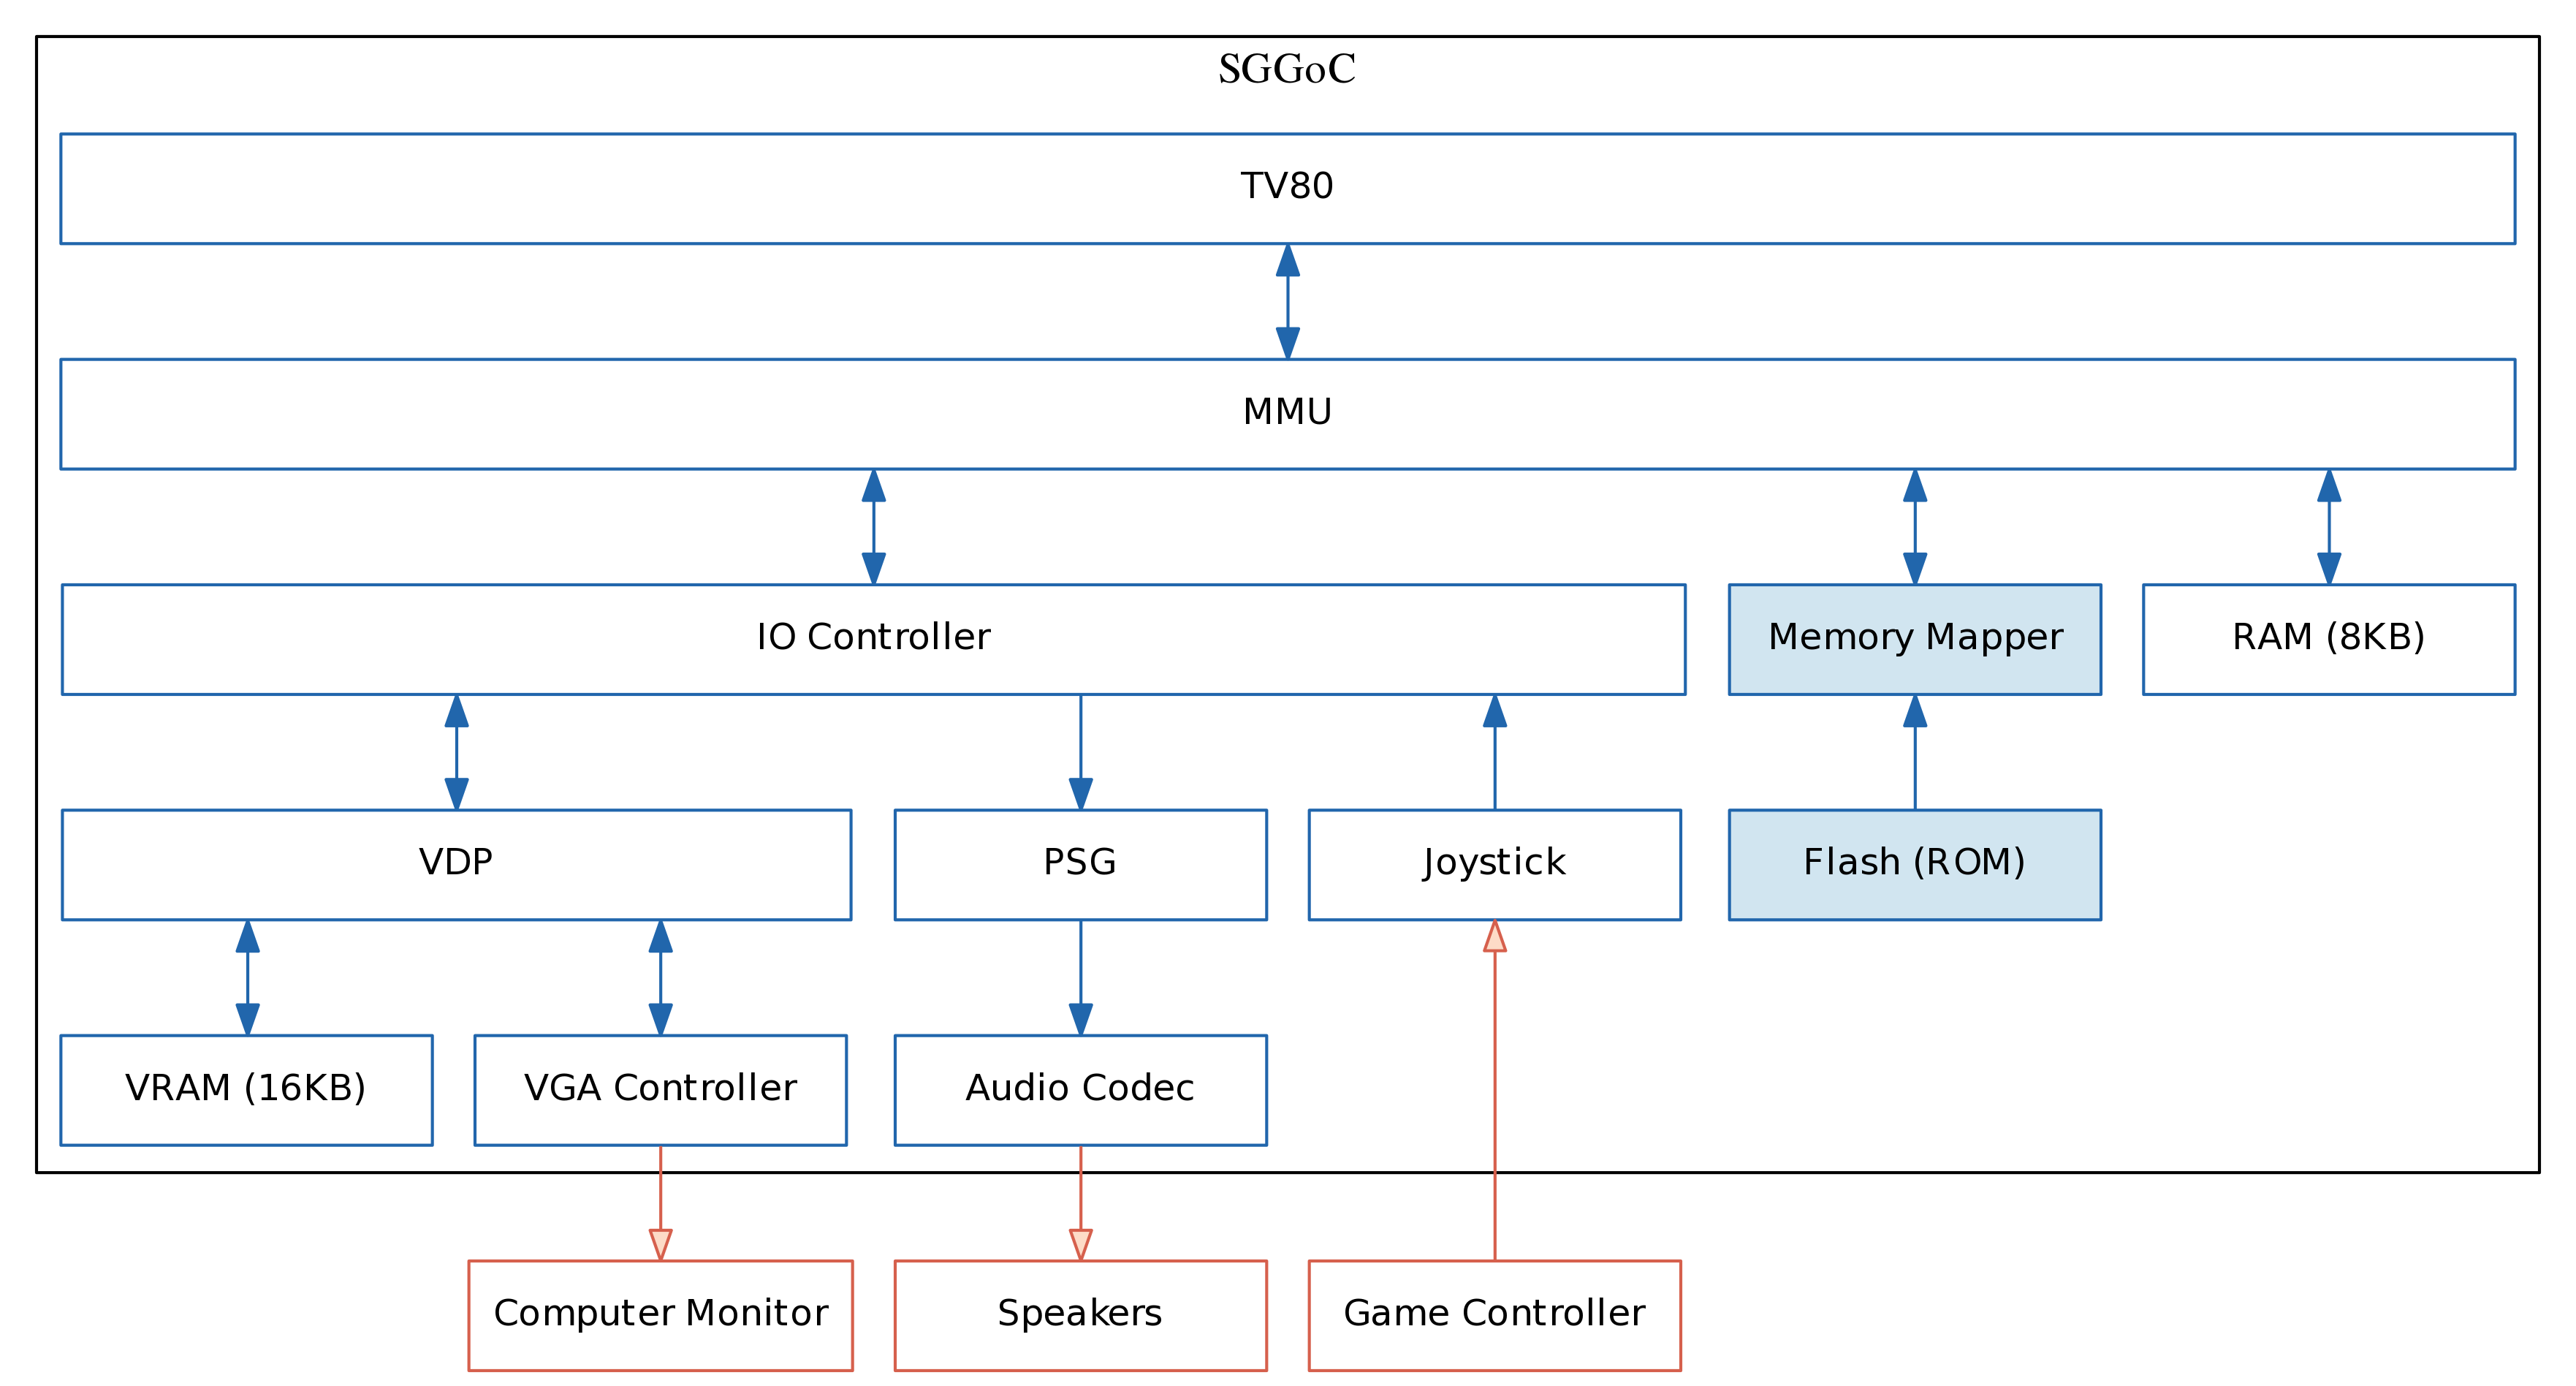
\includegraphics[width=\textwidth]{../block_diagrams/block_diagram_internal_cart.png}
    \end{center}
\end{frame}

\begin{frame}
    \frametitle{Game Cartridge}

    \begin{columns}[c]
        \column{0.5\textwidth}
            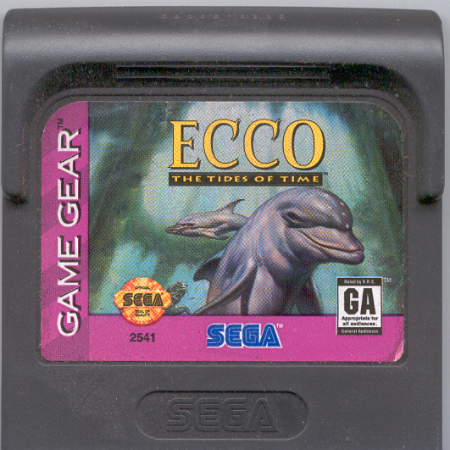
\includegraphics[width=\textwidth]{../design/gg_cart.png}
        \column{0.5\textwidth}
            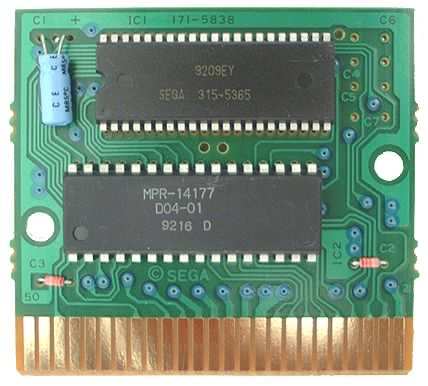
\includegraphics[width=\textwidth]{../design/gg_cart_pcb.png}
    \end{columns}
\end{frame}

\begin{frame}
    \frametitle{Game Cartridge}

    \begin{columns}[c]
        \column{0.5\textwidth}
            Each game cartridge made up of at least two components:
            \begin{itemize}
                \item<2->Game data ROM
                \item<3->Memory Mapper
            \end{itemize}
            \includegraphics<4->[width=\textwidth]{../design/mapper.png}

        \column{0.5\textwidth}
            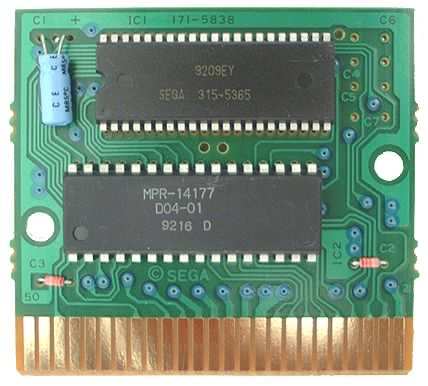
\includegraphics[width=\textwidth]{../design/gg_cart_pcb.png}
    \end{columns}
    \vspace{0.8cm}
    \onslide<5-> {Practically every game ROM has been dumped as is available online}
\end{frame}

\begin{frame}
    \frametitle{Storing Game ROMs}

    A few options to store game ROMs:
    \begin{enumerate}
        \olditem<1->\color<7->{red}Hookup the actual cartridge
        \begin{itemize}
            \olditem<4->Straight forward
            \olditem<5->Don't have to re-implement the memory mappers
            \olditem<6->Defeats most of the point of the project
        \end{itemize}
        \olditem<2->\color<10->{red}Store them on a SD card
        \begin{itemize}
            \olditem<8->Extremely portable / convenient
            \olditem<9->Complicated interface
        \end{itemize}
        \olditem<3->\color<14->{green}Store them on the 4MB flash chip on the DE1
        \begin{itemize}
            \olditem<11->Fairly straightforward
            \olditem<12->Extremely non-portable
            \olditem<13->Flash chip looks just like original ROM chips
        \end{itemize}
    \end{enumerate}
\end{frame}

\begin{frame}
    \frametitle{ROM Flasher Tool}

    Need a tool to load a ROM file into the flash chip from the PC
    \vspace{0.25cm}
    \begin{enumerate}
        \item<2->Load RS232-to-Flash bridge into the FPGA
        \item<3->PC waits for FPGA to request a byte
        \item<4->PC sends the next byte of ROM file
        \item<5->FPGA writes byte to flash
        \item<6->Go back to 2
    \end{enumerate}
    \vspace{0.5cm}
    \onslide<7-> {Can also do the reverse to read back and verify the flash contents against the ROM file}
\end{frame}

\begin{frame}
    \frametitle{ROM Flasher Tool}
    \vspace{0.5cm}
    \begin{columns}[c]
        \column{0.5\textwidth}
            \centering Writing
            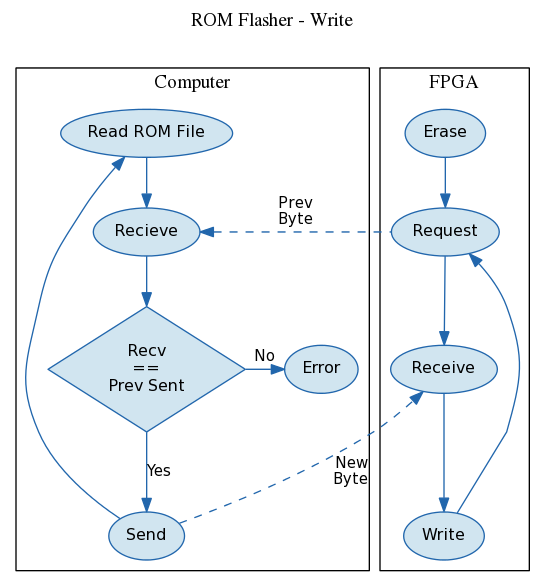
\includegraphics[height=0.65\textheight]{../../fpga/rom_flasher/doc/block_diagram_write.png}
        \column{0.5\textwidth}
            \centering Reading
            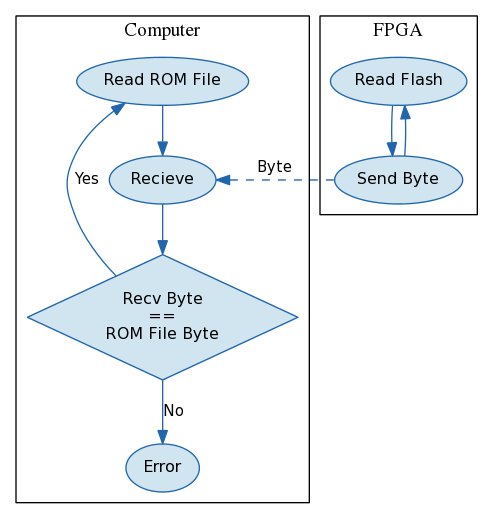
\includegraphics[height=0.65\textheight]{../../fpga/rom_flasher/doc/block_diagram_read.png}
    \end{columns}
\end{frame}

\begin{frame}
    \frametitle{Zilog Z80}
    \begin{center}
        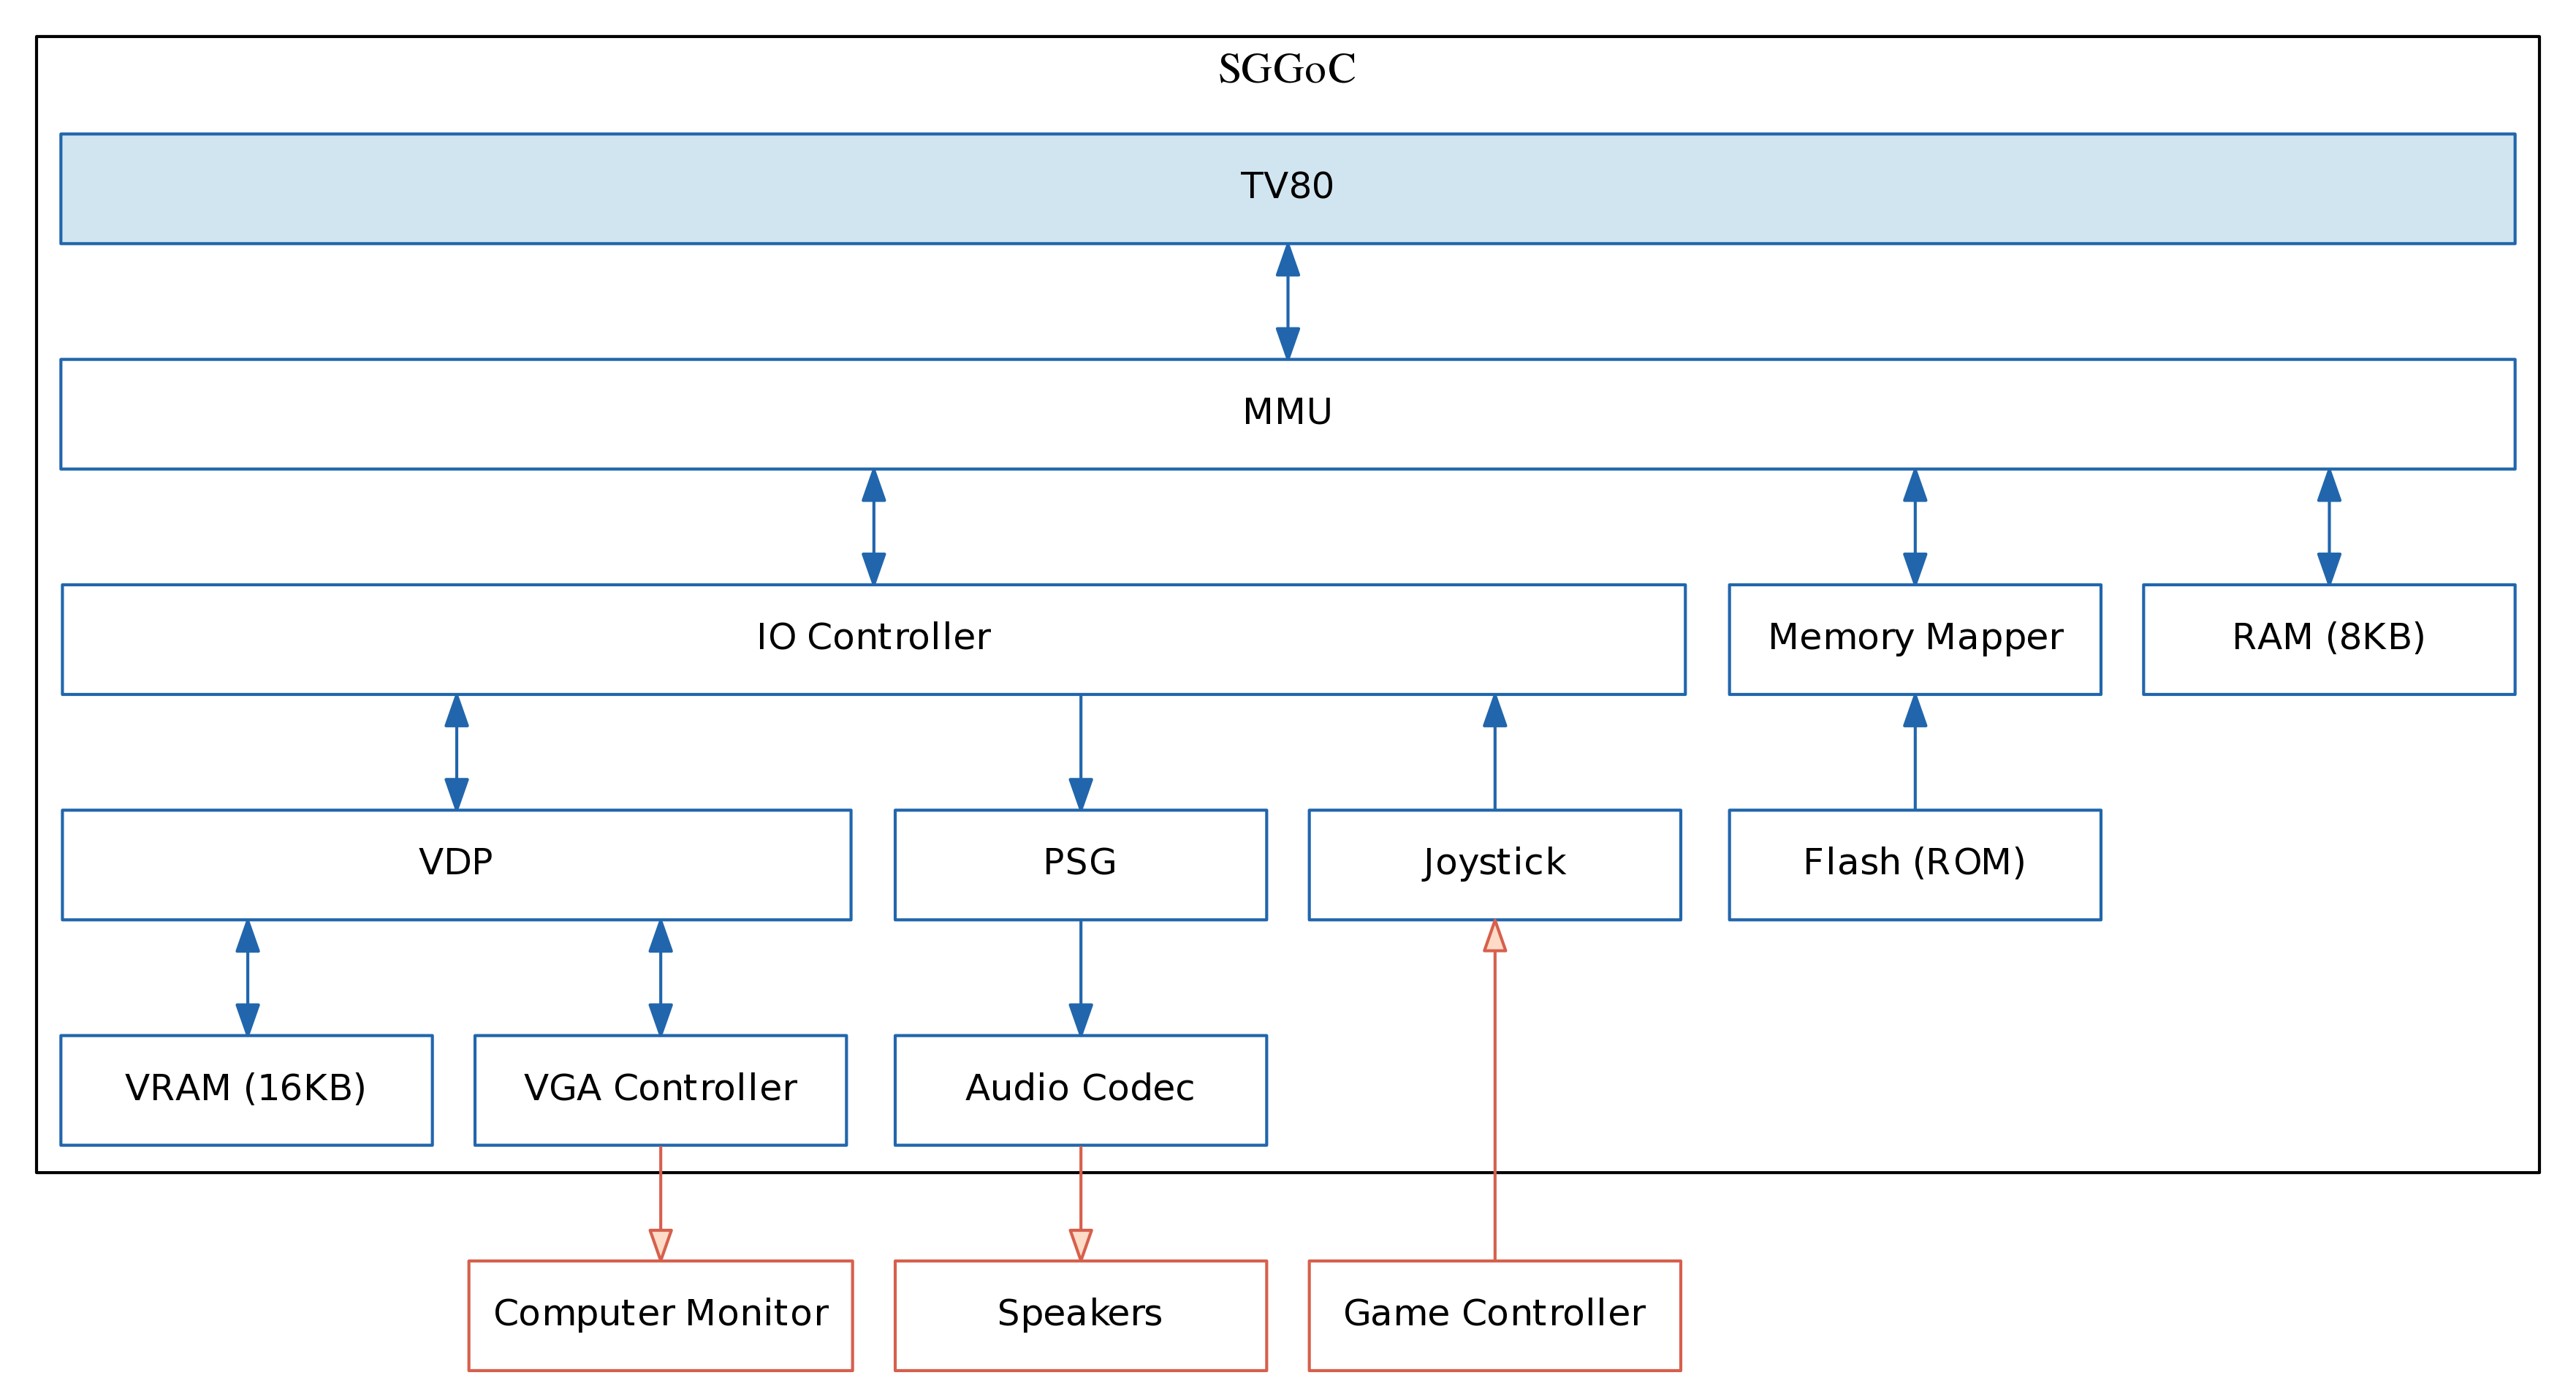
\includegraphics[width=\textwidth]{../block_diagrams/block_diagram_internal_tv80.png}
    \end{center}
\end{frame}

\begin{frame}
    \frametitle{Zilog Z80}

    \begin{columns}[c]
        \column{0.5\textwidth}
        \begin{itemize}
            \item<1-> Implementing a Zilog Z80 is totally outside the scope of this project
            \item<2-> Numerous implementations available online for free
            \item<3-> TV80 is an open source, proven, cycle accurate Z80 implementation written in Verilog
        \end{itemize}

        \column{0.5\textwidth}
            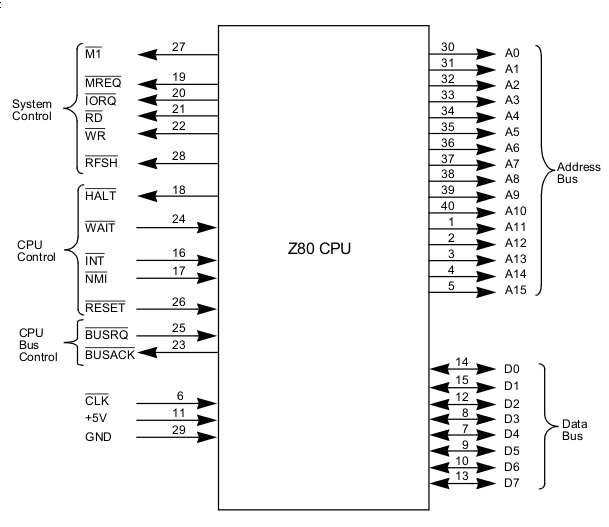
\includegraphics[width=\textwidth]{../design/z80.png}
    \end{columns}
    \vspace{0.5cm}
    \onslide<3-> { \url{http://opencores.org/project,tv80}}

\end{frame}

\begin{frame}
    \frametitle{System and Video RAM}
    \begin{center}
        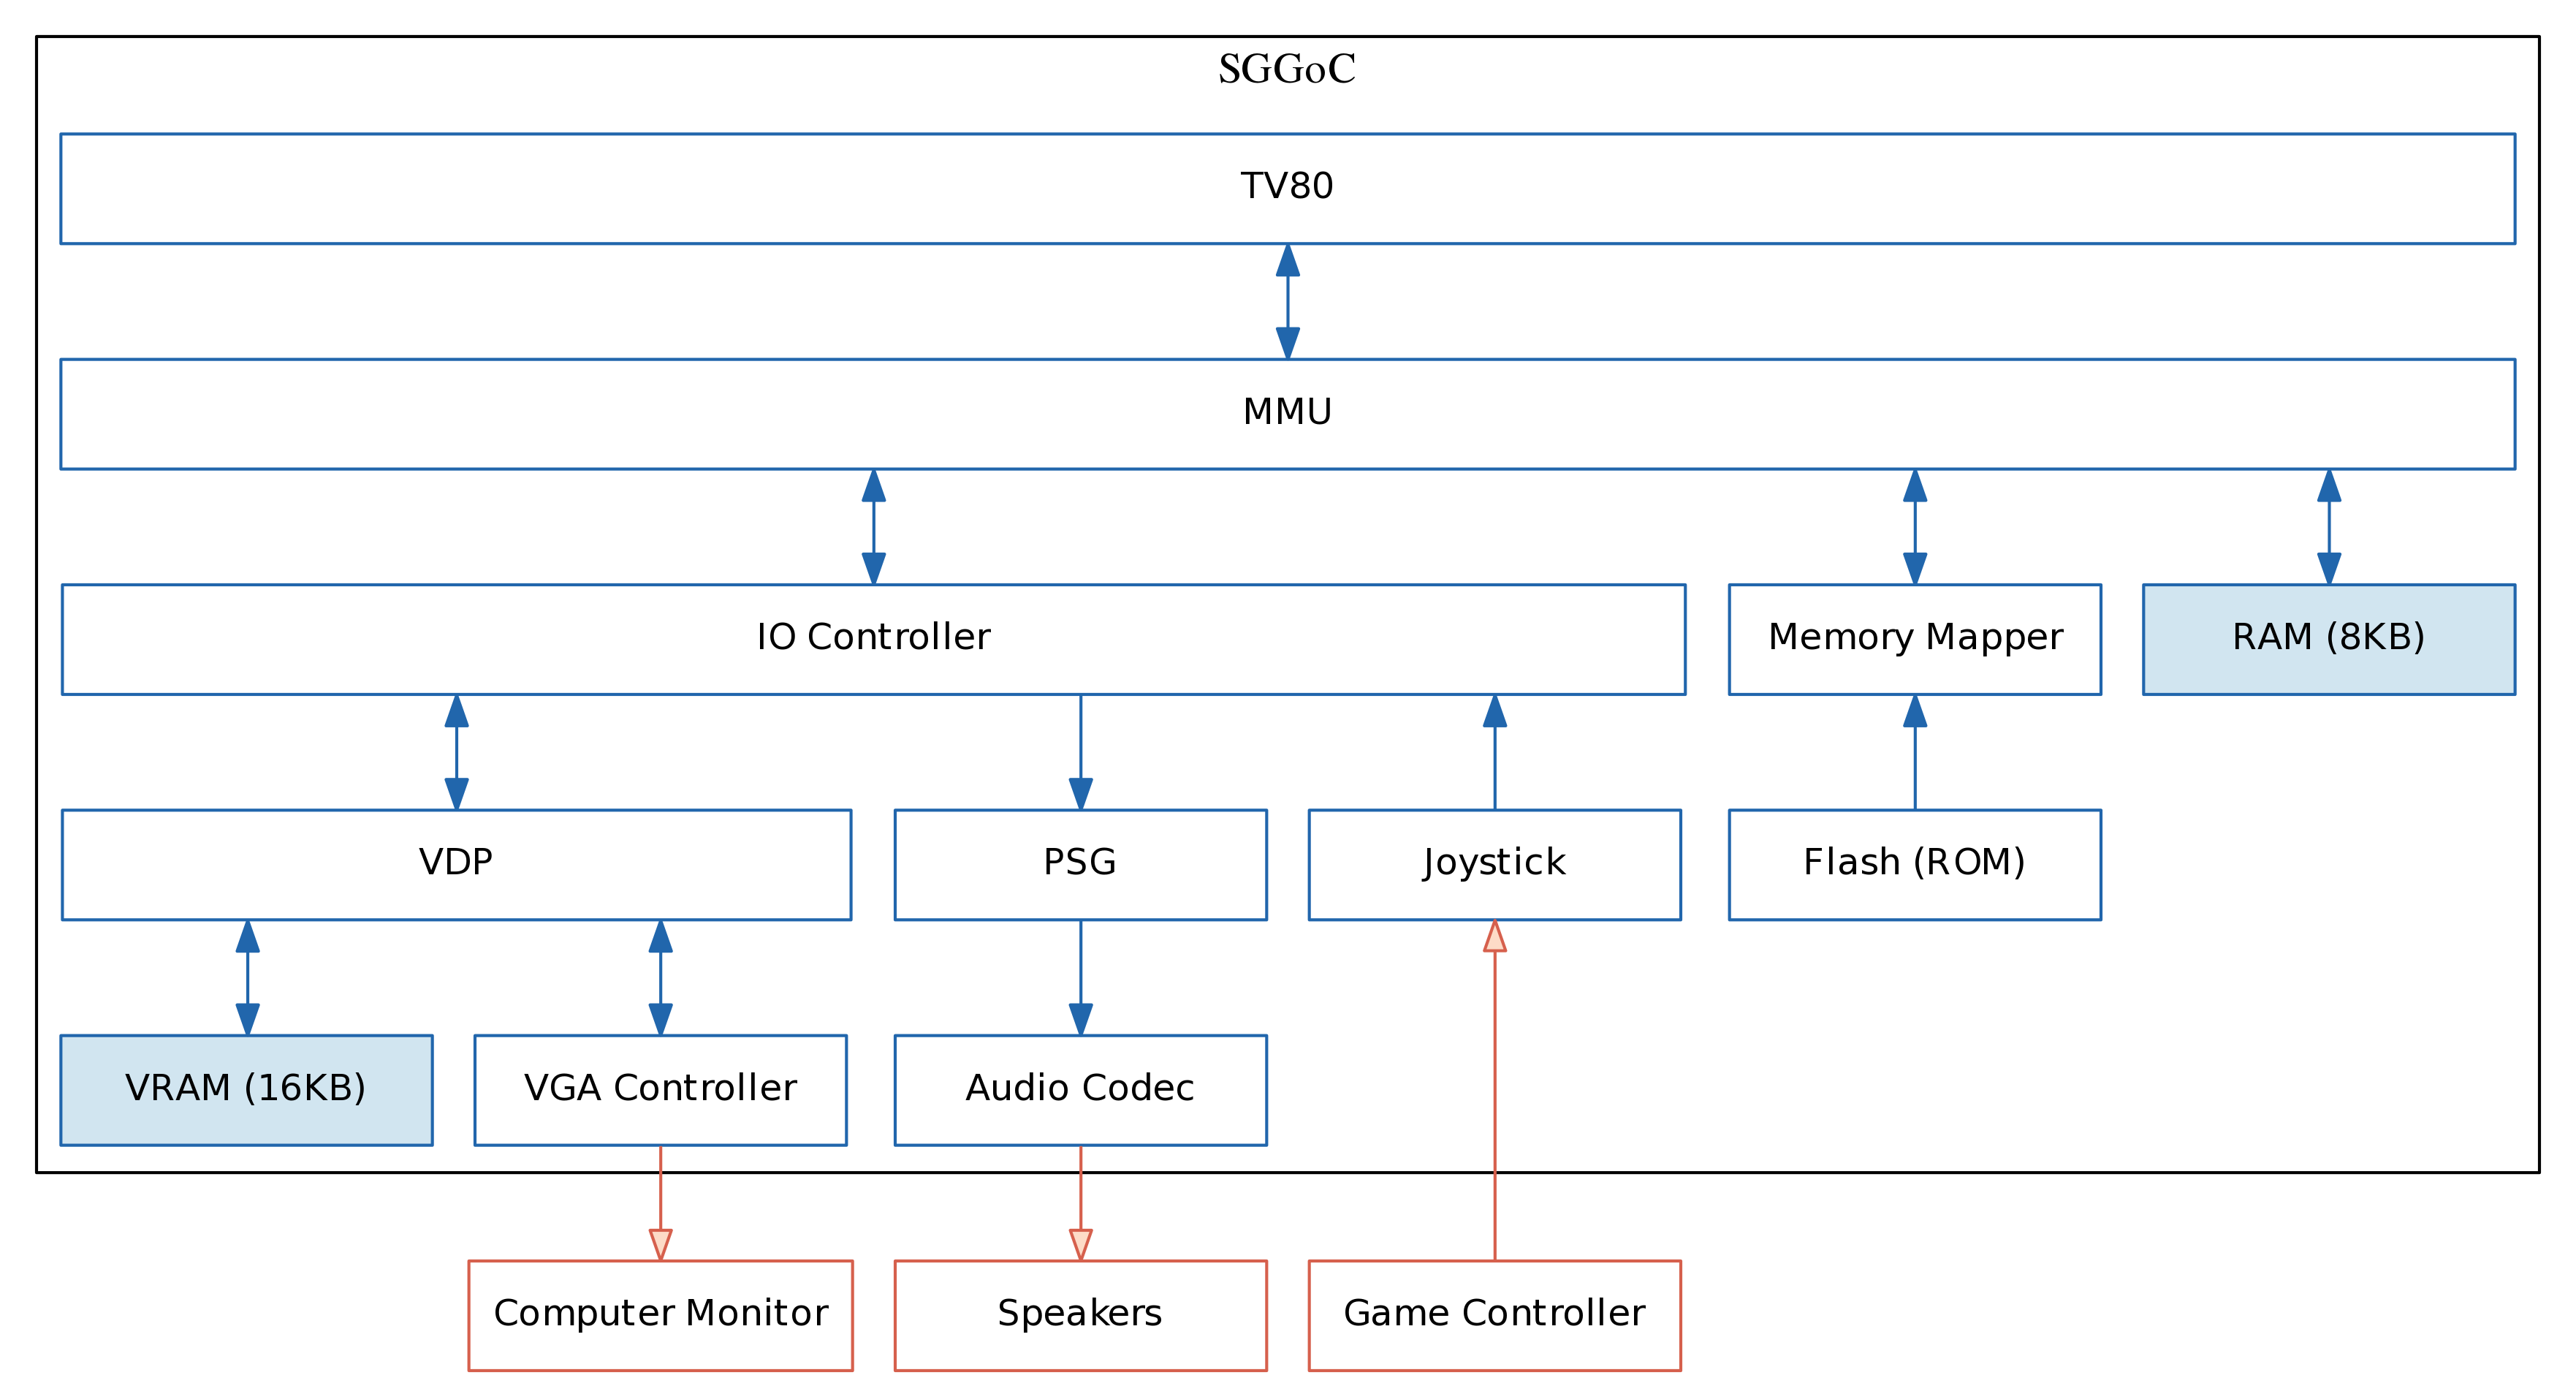
\includegraphics[width=\textwidth]{../block_diagrams/block_diagram_internal_ram.png}
    \end{center}
\end{frame}

\begin{frame}
    \frametitle{System and Video RAM}

    \begin{itemize}
        \item<1-> Most modern FPGAs have more internal RAM than legacy systems
        \item<2-> Cyclon II has enough internal block RAM (30KB) to fit both system and video RAM
        \item<3-> \emph{Design Strategy:} Write code that implies generic block RAM as opposed to device specific
            primitives to increase portability of codebase
    \end{itemize}
    \vspace{0.5cm}
    \onslide<3->{{\small \url{http://danstrother.com/2010/09/11/inferring-rams-in-fpgas/}}}

\end{frame}

\begin{frame}
    \frametitle{Video Display Processor (VDP)}
    \begin{center}
        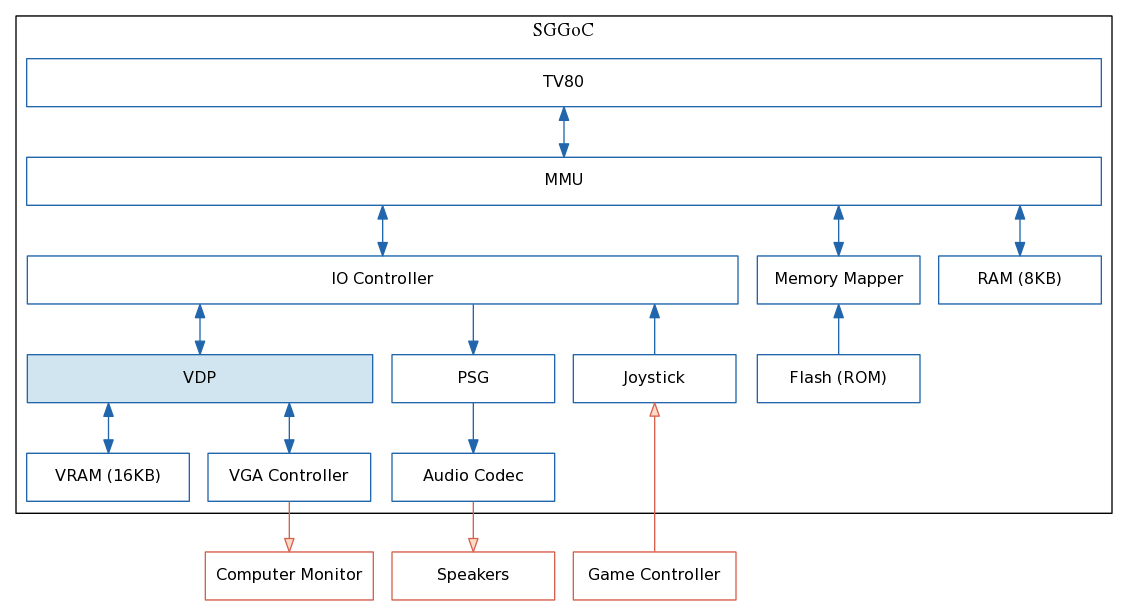
\includegraphics[width=\textwidth]{../block_diagrams/block_diagram_internal_vdp.png}
    \end{center}
\end{frame}

\begin{frame}
    \frametitle{Video Display Processor (VDP)}

    \begin{itemize}
        \item<1-> Texas Instruments TMS9918a
        \item<2-> Used in a number of legacy systems but no good HDL implementation exists online
        \item<3-> Meant to drive CRTs so functionality maps perfectly to the VGA interface on the DE1
        \item<4-> Communicates with the Z80 as an IO device
    \end{itemize}
    \vspace{0.5cm}
    \onslide<1->{{\small \url{http://en.wikipedia.org/wiki/Texas_Instruments_TMS9918}}}

\end{frame}

\section{Testing Strategy}
\begin{frame}
    \frametitle{Testing Strategy}
    Game Gear is hard to test/verify
    \begin{itemize}
            \olditem<2-> Its only output is video (no UART, JTAG, etc..)
            \olditem<3-> Most documentation is 3rd party
    \end{itemize}
    \vspace{0.25cm}
    \onslide<4->{Our strategy:}
    \begin{enumerate}
        \olditem<5-> Use an emulator to watch memory fetches and get memory dumps
        \olditem<6-> Initialize our RAMs with these dumps and verify we achieve the same visual output
        \olditem<7-> Watch instruction fetches with a logic analyzer and see if they match the emulator
    \end{enumerate}
    \vspace{0.25cm}
    \onslide<8->{Could replace emulator with a logic/bus analyzer connected to the original hardware}
\end{frame}

\section{Issues of Concern}
\begin{frame}
    \frametitle{Issues of Concern}
    \begin{itemize}
        \item Each component is tightly dependant on each other. Need to implement each one
        correctly for whole system to function.
        \item If something doesn't work we cannot simply change the design spec. We are working
            against an established spec that cannot be changed.
    \end{itemize}
\end{frame}

\begin{frame}
\frametitle{}
    \begin{center}
        \Huge
        Questions?
    \end{center}
\end{frame}

\end{document}
